%%%%%%%%%%%%%%%%%%%%%%%%%%%%%%%%%%%%%%%%%%%%%%%%%%%
%% LaTeX book template                           %%
%% Author:  Amber Jain (http://amberj.devio.us/) %%
%% License: ISC license                          %%
%%%%%%%%%%%%%%%%%%%%%%%%%%%%%%%%%%%%%%%%%%%%%%%%%%%

\documentclass[a4paper,12pt]{book}
\usepackage{iftex}
\ifPDFTeX
  % PDFLaTeX or LaTeX 
  \usepackage[utf8]{inputenc}
  \usepackage[T1]{fontenc}
  \DeclareUnicodeCharacter{00B5}{\ensuremath{\mu}}
\else
  %  XeLaTeX or LuaLaTeX
  \usepackage{fontspec}
\fi
%\usepackage[T1]{fontenc}
%\usepackage[utf8]{inputenc}
\usepackage[left=2cm,right=1cm,top=2cm,bottom=2cm,headheight=1cm]{geometry}
\usepackage{lmodern}
\usepackage{amsmath}
\usepackage{textcomp}
\usepackage{multicol}
\usepackage[]{ragged2e}
\usepackage[dvipsnames]{xcolor}

%%%%%
\usepackage[12pt]{moresize}
%\fontsize{8}{20}\selectfont
\usepackage{amssymb}
\usepackage{enumerate}
%%%%%
\usepackage{pifont}
\usepackage{braket}
\usepackage{esint}
\usepackage{ziffer}
\usepackage{latexsym}
\usepackage[normalem]{ulem}
\usepackage{color,tikz}
\usepackage{mathtools}
\usepackage{setspace}
\usepackage{tocloft}
\usepackage{longtable}
\usepackage{url}
\usepackage{booktabs}
\usepackage{float}
\usepackage{graphicx, nicefrac}
\usepackage{scalefnt}
\usepackage{tikz}
\usetikzlibrary{decorations.pathmorphing}
\usetikzlibrary{shapes.geometric, arrows}
\usepackage[ruled, vlined, linesnumbered]{algorithm}
\usepackage{caption}%
\usepackage[Sonny]{fncychap}
\usepackage[weather, clock]{ifsym}
\usepackage[most]{tcolorbox}
%%%%%%%%%%%%%%%%%%%%%%%%%%%%%%%%%%%%%%%%%%%%%%%%%%%%%%%%%
% Configurações para o Maxima %
%%%%%%%%%%%%%%%%%%%%%%%%%%%%%%%%%%%%%%%%%%%%%%%%%%%%%%%%%


%\usepackage{graphicx}

\usepackage{grffile}
\usepackage{ifthen}
\newsavebox{\picturebox}
\newlength{\pictureboxwidth}
\newlength{\pictureboxheight}
\newcommand{\includeimage}[1]{
    \savebox{\picturebox}{\includegraphics{#1}}
    \settoheight{\pictureboxheight}{\usebox{\picturebox}}
    \settowidth{\pictureboxwidth}{\usebox{\picturebox}}
    \ifthenelse{\lengthtest{\pictureboxwidth > .95\linewidth}}
    {
        \includegraphics[width=.95\linewidth,height=.80\textheight,keepaspectratio]{#1}
    }
    {
        \ifthenelse{\lengthtest{\pictureboxheight>.80\textheight}}
        {
            \includegraphics[width=.95\linewidth,height=.80\textheight,keepaspectratio]{#1}
            
        }
        {
            \includegraphics{#1}
        }
    }
}
\newlength{\thislabelwidth}
\DeclareMathOperator{\abs}{abs}

\definecolor{labelcolor}{RGB}{100,0,0}



%%%%%%%%%%%%%%%%%%%%%%%%%%%%%%%%%%%%%%%%%%%%%%%%%%%%%%%%%
% Source: http://en.wikibooks.org/wiki/LaTeX/Hyperlinks %
%%%%%%%%%%%%%%%%%%%%%%%%%%%%%%%%%%%%%%%%%%%%%%%%%%%%%%%%%
\usepackage{hyperref}
%\usepackage{graphicx}
\usepackage[portuguese]{babel}

%%%%%%%%%%%%%%%%%%%%%%%%%%%%%%%%%%%%%%%%%%%%%%%%%%%%%%%%%%%%%%%%%%%%%%%%%%%%%%%%
% 'dedication' environment: To add a dedication paragraph at the start of book %
% Source: http://www.tug.org/pipermail/texhax/2010-June/015184.html            %
%%%%%%%%%%%%%%%%%%%%%%%%%%%%%%%%%%%%%%%%%%%%%%%%%%%%%%%%%%%%%%%%%%%%%%%%%%%%%%%%
\newenvironment{dedication}
{
   \cleardoublepage
   \thispagestyle{empty}
   \vspace*{\stretch{1}}
   \hfill\begin{minipage}[t]{0.66\textwidth}
   \raggedright
}
{
   \end{minipage}
   \vspace*{\stretch{3}}
   \clearpage
}

%%%%%%%%%%%%%%%%%%%%%%%%%%%%%%%%%%%%%%%%%%%%%%%%
% Chapter quote at the start of chapter        %
% Source: http://tex.stackexchange.com/a/53380 %
%%%%%%%%%%%%%%%%%%%%%%%%%%%%%%%%%%%%%%%%%%%%%%%%
\makeatletter
\renewcommand{\@chapapp}{}% Not necessary...
\newenvironment{chapquote}[2][2em]
  {\setlength{\@tempdima}{#1}%
   \def\chapquote@author{#2}%
   \parshape 1 \@tempdima \dimexpr\textwidth-2\@tempdima\relax%
   \itshape}
  {\par\normalfont\hfill--\ \chapquote@author\hspace*{\@tempdima}\par\bigskip}
\makeatother


%%%%%%%%%%%%%%%%%%%%%%%%%%%%%%%%%%%%%%%%%%%%%%%%%%%
% First page of book which contains 'stuff' like: %
%  - Book title, subtitle                         %
%  - Book author name                             %
%%%%%%%%%%%%%%%%%%%%%%%%%%%%%%%%%%%%%%%%%%%%%%%%%%%

% Book's title and subtitle
\title{\Huge \textbf{\MakeUppercase{Simulações de Ondulatória com Uso do Maxima}} \footnote{This is a footnote.} \\  }
% Author
\author{\textsc{Elielzer Nuayed}\thanks{\url{https://github.com/elielzer}}}


\begin{document}

\frontmatter
\maketitle

%%%%%%%%%%%%%%%%%%%%%%%%%%%%%%%%%%%%%%%%%%%%%%%%%%%%%%%%%%%%%%%
% Add a dedication paragraph to dedicate your book to someone %
%%%%%%%%%%%%%%%%%%%%%%%%%%%%%%%%%%%%%%%%%%%%%%%%%%%%%%%%%%%%%%%
\begin{dedication}
Dedicated to Calvin and Hobbes.
\end{dedication}

%%%%%%%%%%%%%%%%%%%%%%%%%%%%%%%%%%%%%%%%%%%%%%%%%%%%%%%%%%%%%%%%%%%%%%%%
% Auto-generated table of contents, list of figures and list of tables %
%%%%%%%%%%%%%%%%%%%%%%%%%%%%%%%%%%%%%%%%%%%%%%%%%%%%%%%%%%%%%%%%%%%%%%%%
{\tableofcontents}
{\listoffigures}
{\listoftables}

\mainmatter

%%%%%%%%%%%
% Preface %
%%%%%%%%%%%
\chapter*{Preface}
Este livro foi concebido a partir de um \emph{insight} pessoal após eu ler um anúncio sobre uso do \emph{Maxima} no ensino da Física. Então veio-me a ideia de escrever algo nesse sentido.
Escolhi sobre ondulatória. O Maxima é introduzido no contexto como ambiente de apoio no momento que seja necessário simular as proposições. Dentre as proposições abordaremos situações clássicas, pois o objetivo é justamente apresentar o cartel de ferramentas desse software adequadas para transcrever a linguagem da física para representar as situações problema.



%%%%%%%%%%%%%%%%
% NEW CHAPTER! %
%%%%%%%%%%%%%%%%
\chapter{INTRODUÇÃO}

\begin{chapquote}{Author's name, \textit{Source of this quote}}
``This is a quote and I don't know who said this.''
\end{chapquote}

\section{Um Pouco Sobre Ondas}
Há várias situações no dia a dia nas quais as coisas acontecem repentinamente, ou inesperadamente, vindo, depois a cessar seus efeitos, ou, em outros casos, repercutem mais além. É comum nos referirmos a isso com a expressão: "isso é apenas uma onda, logo passará". Isso, claro, devido a que tais situações são transitórias, exemplos: pandemias, endemias, o preço de commodities, tsunamis, terremotos, até notícias ou eventos cotidianos. Algumas vezes tais situações apresentam comportamento oscilante, como na superfície de um líquido em uma piscina, ou mesmo em fontes naturais de água, como em rios, mares e oceanos durante a passagem de uma embarcação.

É importante notar que existem características diferentes em tais situações. Alguns simplesmente oscilam ou vibram e em outros casos, além de oscilar ou vibrar, essa condição é posteriormente transmitida para outros locais do ambiente onde tais situações ocorrem. Neste segundo caso, diz-se que há uma propagação do fenômeno. De tal forma que, oscilação, onda, propagação são termos correlacionados.

Etimologicamente, a palavra onda teria a ver com o significado de algo que flutua na água. As descobertas e desenvolvimentos neste tema em seus primórdios derivaram do estudo dos sons musicais. Diz-se que o estudo moderno de ondas e acústica se originou com \emph{Galileu Galilei}.

A figura \ref{fig:mapa.ondas} apresenta a evolução, numa perspectiva histórica, do conhecimento científico desta temática, através da contribuição de vários investigadores.

\begin{figure}[htbp!]
    \centering
    \caption{Representação da evolução do conhecimento sobre ondas.}
        \label{fig:mapa.ondas}
    %\begin{Center}
    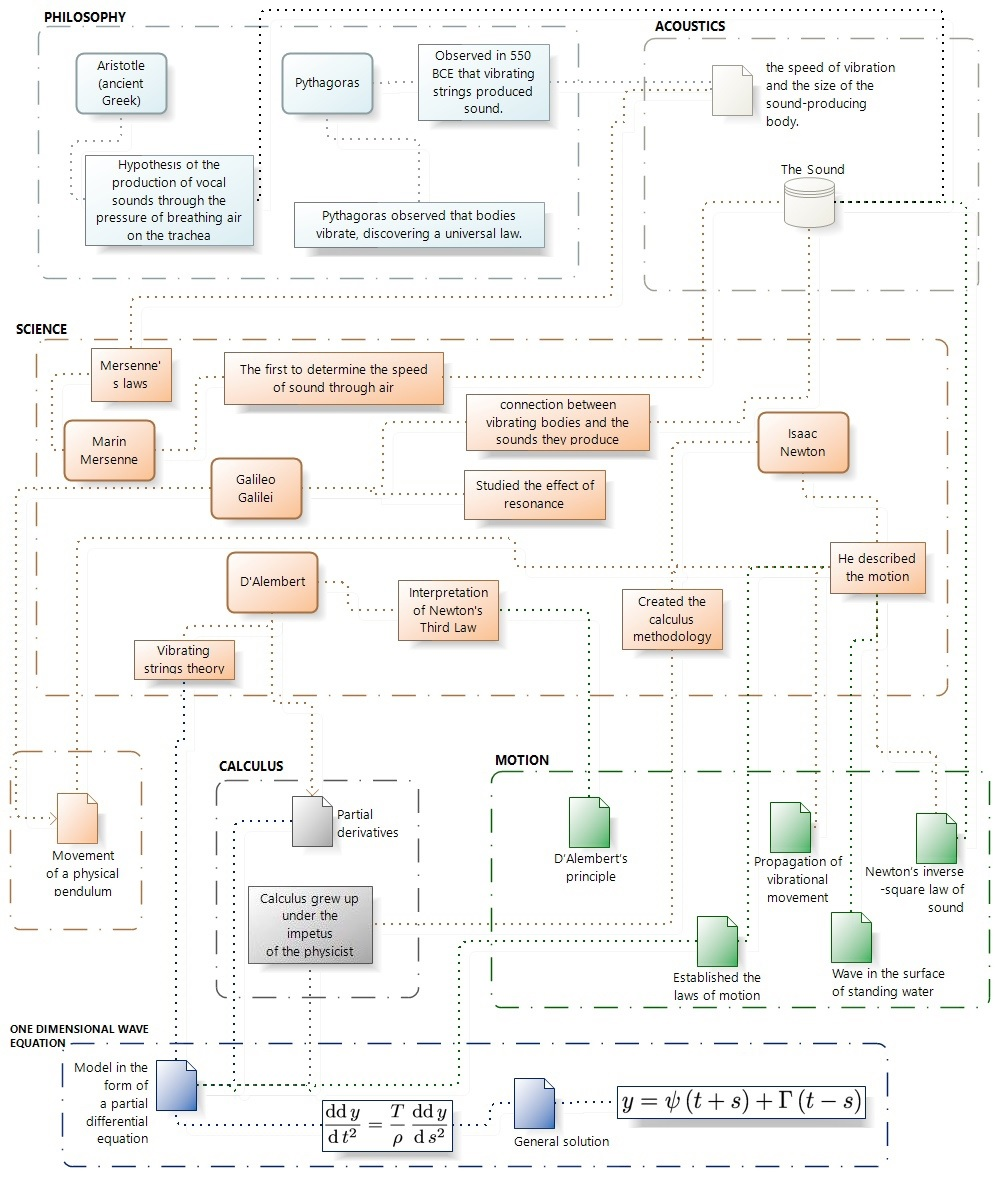
\includegraphics[width=0.95\textwidth,height=0.95\textheight]{sounds.jpg}
	%\end{Center}
\end{figure}

\newpage
\section{Sobre o Maxima}
De acordo com descrição no site fabricante, o Maxima é um programa de computador do tipo multiplataforma, ou seja, ele está preparado para trabalhar (compilar) sob diversos sistemas operacionais ou plataformas computacionais.
Ainda de acordo com esse site o Maxima é uma versão evoluída de software especialista Macsyma. Os sistemas especialistas foram criados com a finalidade de reproduzir o raciocínio ou expertise de um  profissional de alguma área de conhecimento específica.

Assm,o Maxima é um sistema especialista para a manipulação de expressões matemáticas, tanto na forma simbólica como na forma numérica, incluindo:
\begin{itemize}
    \item diferenciação,
    \item integração,
    \item séries de Taylor,
    \item transformadas de Laplace,
    \item equações diferenciais ordinárias,
    \item sistemas de equações lineares,
    \item polinômios,
    \item conjuntos,
    \item listas,
    \item vetores,
    \item matrizes e
    \item tensores.
\end{itemize}

\noindent O que caracteriza a matemática simbólica é de não estar atrelada a um determinado idioma, por exemplo a expressão algébrica: \(x+2=7\), tem o mesmo significado em qualquer idioma. Portanto o Maxima é um sistema algébrico computacional para auxílio no cálculo e manipulação da  matemática simbólica visado simplificar o esforço de trabalho do estudante ou profissional (professor ou pesquisador).

O Maxima produz também resultados numéricos de alta precisão usando frações exatas, inteiros de precisão arbitrária e números de ponto flutuante de precisão variável. O Maxima pode plotar funções e dados em duas e três dimensões. Utilizaremos em nossos desenvolvimentos a plataforma gráfica do wxMaxima\textregistered .

%%%%%%%%%%%%%%%%%%%%%%%%%%%%%%%%%%%%%%%%%%%%%%%%%%%%%%%
% Sample table                                        %
% Source: www1.maths.leeds.ac.uk/latex/TableHelp1.pdf %
%%%%%%%%%%%%%%%%%%%%%%%%%%%%%%%%%%%%%%%%%%%%%%%%%%%%%%%
\begin{table}[ht]
\caption{Sample table} % title of Table
\centering % used for centering table
\begin{tabular}{c c c c}
% centered columns (4 columns)
\hline\hline %inserts double horizontal lines
S. No. & Column\#1 & Column\#2 & Column\#3 \\ [0.5ex]
% inserts table
%heading
\hline % inserts single horizontal line
1 & 50 & 837 & 970 \\
2 & 47 & 877 & 230 \\
3 & 31 & 25 & 415 \\
4 & 35 & 144 & 2356 \\
5 & 45 & 300 & 556 \\ [1ex] % [1ex] adds vertical space
\hline %inserts single line
\end{tabular}
\label{table:nonlin} % is used to refer this table in the text
\end{table}
\section{Como Instalar o wxMaxima\textregistered}
Instalar um software é uma tarefa que a maioria de usuários de PC já fizeram alguma vez, e instalar o Maxima é uma tarefa que não haverá muita dificuldade. O primeiro passo é obter o arquivo instalador. Uma opção é fazer o processo de \emph{download} do endereço da internet ou URL (sugestão do autor): maxima.sourceforge.io/windows-install.html (\ref{fig:site-maxima}). 
\begin{figure}[htbp!]
    \centering
    \caption{Entrando com a URL, para buscar a página do Maxima no \emph{Google}.}
        \label{fig:site-maxima}
    %\begin{Center}
    
\includegraphics[]{site-maxima.jpg}
	%\end{Center}
\end{figure}

\noindent A página na figura \ref{fig:pagina-maxima} contém um passo a passo, que é recomendável que seja lido. Entretando, por ora seguiremos mais focados no processo operacional de instalação em si. 
Assim, localize o link, nessa página com o texto: \href{sourceforge.net/projects/maxima/files/Maxima-Windows/5.46.0-Windows/}{5.46.0-Windows}, como mostrado nessa imagem.

\begin{figure}[htbp!]
    \centering
    \caption{Página encontrada do Maxima no navegador da Internet.}
        \label{fig:pagina-maxima}
    %\begin{Center}
    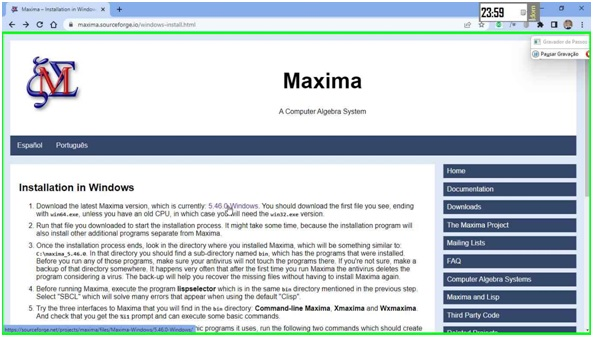
\includegraphics[]{pagina-maxima.jpg}
	%\end{Center}	
\end{figure}
\newpage
\noindent	Como forma de gerenciar o processo de instalação são apresentadas a seguir as janelas que interagem nas diversa etapas dessa instalação.
	\begin{figure}[htbp!]
    \centering
    \caption{Janela que apresenta o início do processo de instalação.}
        \label{fig:maxima-ist-1}
    %\begin{Center}
    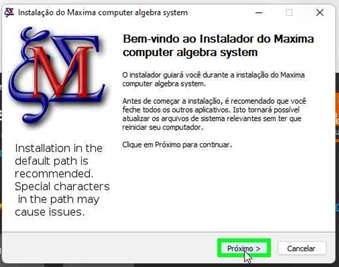
\includegraphics[]{maxima-ist-1.jpg}
	%\end{Center}
\end{figure}


	\begin{figure}[htbp!]
    \centering
    \caption{Janela que apresenta os termos de uso.}
        \label{fig:maxima-ist-2}
    %\begin{Center}
    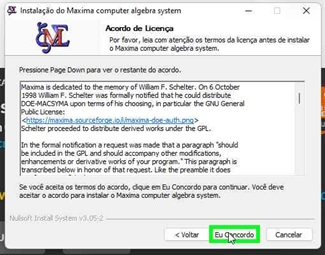
\includegraphics[]{maxima-ist-2.jpg}
	%\end{Center}
\end{figure}

	\begin{figure}[htbp!]
    \centering
    \caption{Janela que apresenta o diretório local para instalação de arquivos.}
        \label{fig:maxima-ist-3}
    %\begin{Center}
    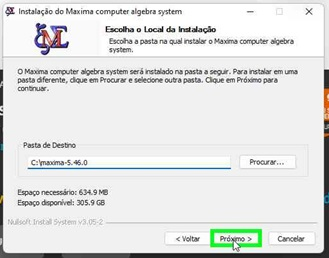
\includegraphics[]{maxima-ist-3.jpg}
	%\end{Center}
\end{figure}

	\begin{figure}[htbp!]
    \centering
    \caption{Janela de configuração de atalhos.}
        \label{fig:maxima-ist-4}
    %\begin{Center}
    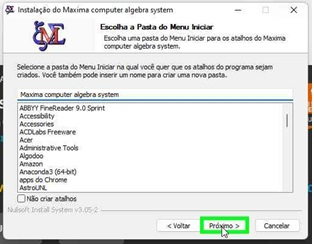
\includegraphics[]{maxima-ist-4.jpg}
	%\end{Center}
\end{figure}

	\begin{figure}[htbp!]
    \centering
    \caption{Janela de configuração do escopo de funções do programa.}
        \label{fig:maxima-ist-5}
    %\begin{Center}
    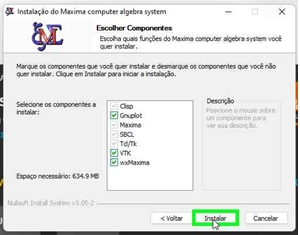
\includegraphics[]{maxima-ist-5.jpg}
	%\end{Center}
\end{figure}

	\begin{figure}[htbp!]
    \centering
    \caption{Janela de status do processo de instalação.}
        \label{fig:maxima-ist-6}
    %\begin{Center}
    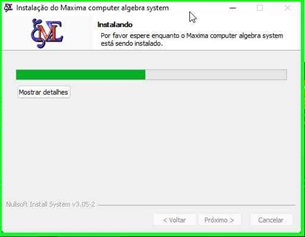
\includegraphics[]{maxima-ist-6.jpg}
	%\end{Center}
\end{figure}

	\begin{figure}[htbp!]
    \centering
    \caption{Janela de confirmação da instalação.}
        \label{fig:maxima-ist-7}
    %\begin{Center}
    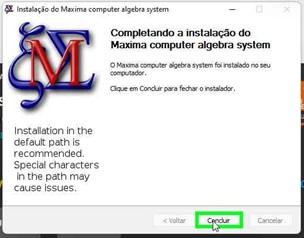
\includegraphics[]{maxima-ist-7.jpg}
	%\end{Center}
\end{figure}

	\begin{figure}[htbp!]
    \centering
    \caption{Aspecto do comando de menu na janela inicial do Windows.}
        \label{fig:menu-windows}
    %\begin{Center}
    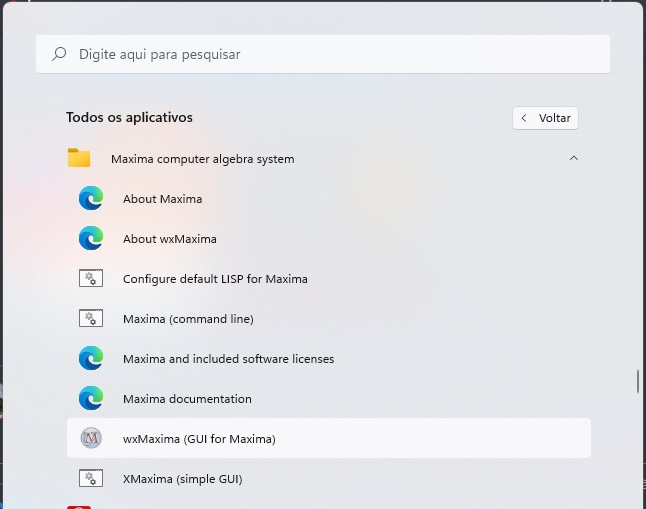
\includegraphics[scale=0.7]{menu-windows.jpg}
	%\end{Center}
\end{figure}
\newpage
\section{Conhecendo a \emph{Interface} Gráfica do wxMaxima}
A janela do aplicativo Maxima é idêntica a um editor de texto, e permite criar um arquivo, abrir um existente e salvar suas alterações, tudo a partir de um um menu supenso de comandos. Ao abrir a janela do aplicativo, esta já fornece de imediato, um prompt para a entrada de comandos de programação, ou textos descritivos, figura \ref{fig:tela-inicial}. A janela do aplicativo Maxima é idêntica a um editor de texto, porém sua funcionalidade lógica é identica á de uma planilha de cálculo, ou seja as janela possui uma estrutura baseada em células de cálculo.

	\begin{figure}[h]
    \centering
    \caption{Aspecto da janela do aplicativo Maxima.}
        \label{fig:tela-inicial}
    %\begin{Center}
    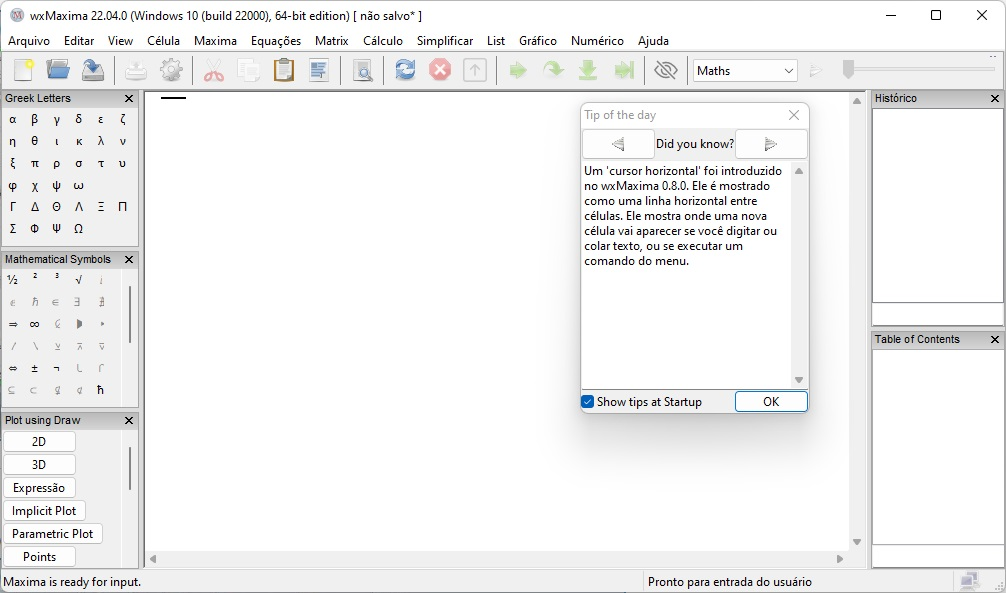
\includegraphics[scale=0.6]{tela-inicial.jpg}
	%\end{Center}
\end{figure}

\noindent A figura \ref{fig:selecao-tipos} mostra o recurso para escolher a opção de tipo de entrada no prompt, que podem ser
\begin{multicols}{2}
\begin{itemize}
\item tipo Texto
\item tipo Math
\item tipo Título
\item tipo Seção
\item tipo Subseção
\item tipo Subsubseção
\item head 5
\item head 6
\end{itemize}
\begin{figure}[H]
    %\centering
    \caption{Pré-seleção de tipo de entrada a ser inserida no prompt.}
        \label{fig:selecao-tipos}
    \begin{Center}
    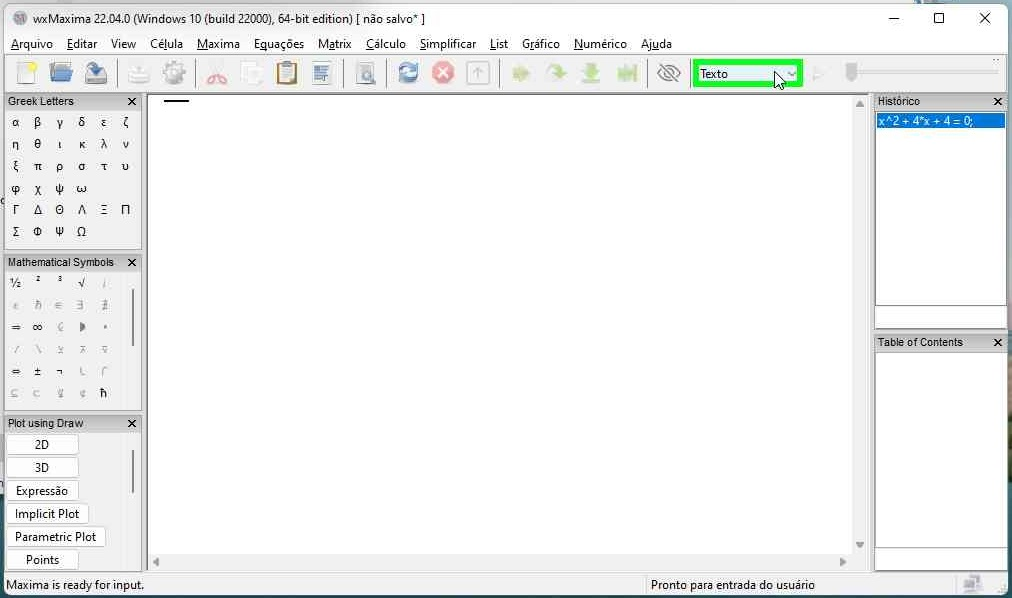
\includegraphics[scale=0.3]{selecao-tipos.jpg}
		\end{Center}
\end{figure}
\end{multicols}
%

\pagebreak
\noindent A figura \ref{fig:selecao-texto} mostra como escolher as opções de tipo de entrada no prompt para o caso de texto. Já a figura \ref{fig:selecao-math} mostra como escolher as opções de tipo de entrada no prompt para o caso de expressão algébrica.
	\begin{figure}[ht!]
    \centering
    \caption{Pré-seleção para inserir texto no prompt.}
        \label{fig:selecao-texto}
    %\begin{Center}
    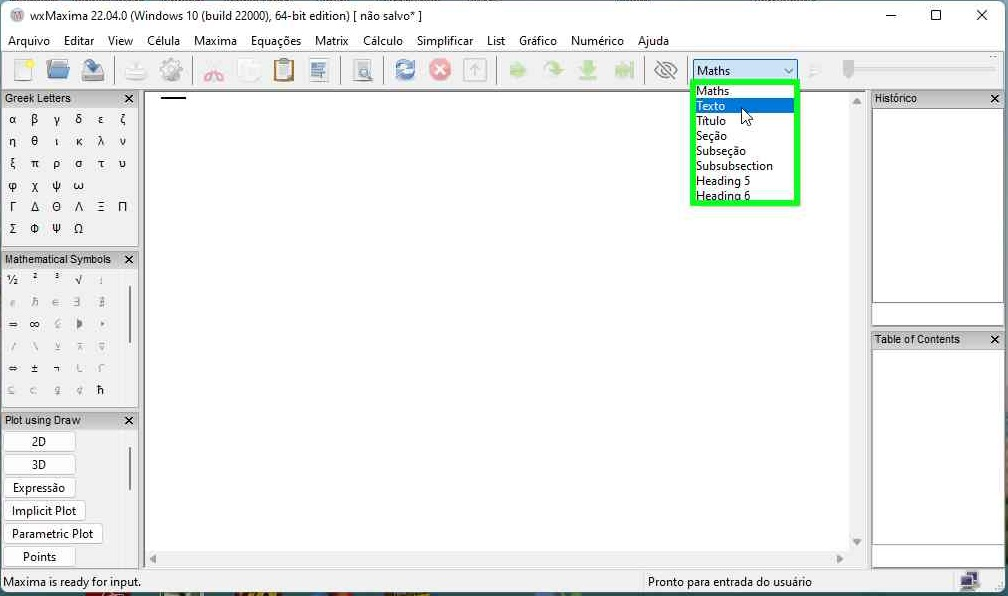
\includegraphics[scale=0.6]{selecao-texto.jpg}
	%\end{Center}
\end{figure}

\begin{figure}[H]
    \centering
    \caption{Pré-seleção para inserir expressão algébrica no prompt.}
        \label{fig:selecao-math}
    %\begin{Center}
    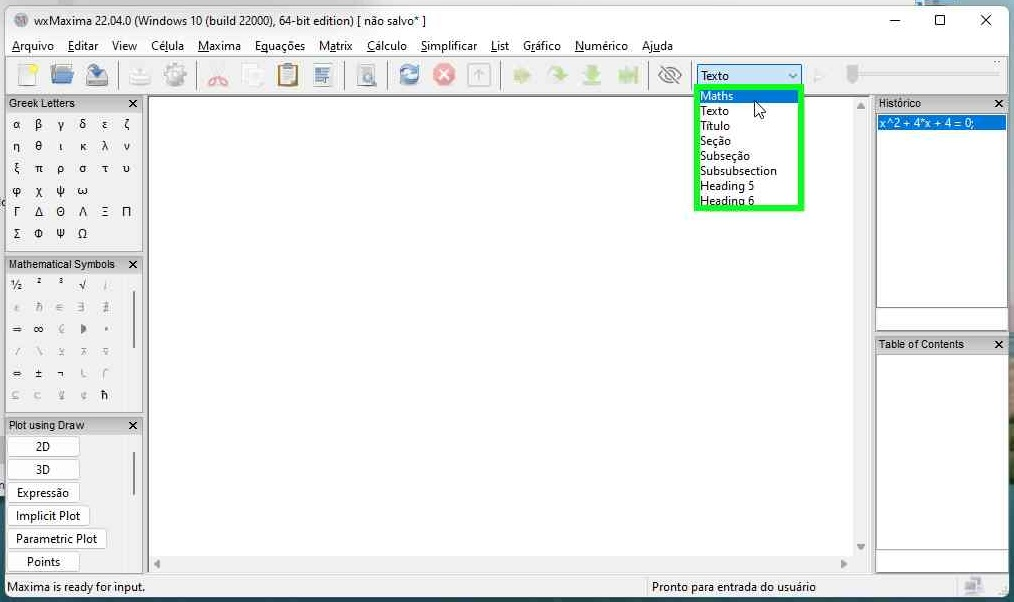
\includegraphics[scale=0.6]{selecao-math.jpg}
	%\end{Center}
\end{figure}
\pagebreak
Até agora nos ativemos a apresentar generalidades que subsidiarão o leitor durante sua jornada no aprendizado ou mesmo na utilização das técnica aqui apresntadas de simulação no Maxima. Assunto que será objeto dos próximos capítulos.

\chapter{TRABALHANDO COM O MAXIMA}
Vamos tomar como primeiro exemplo a fórmula do teorema de Pitágoras. Vamos escrever no \emph{prompt} a seguinte expressão: \textsf{c\^\ 2+b\^\ 2=a\^\ 2}
\begin{figure}[H]
    \centering
    \caption{Entrando uma expressão algébrica.}
        \label{fig:pitagoras}
    %\begin{Center}
    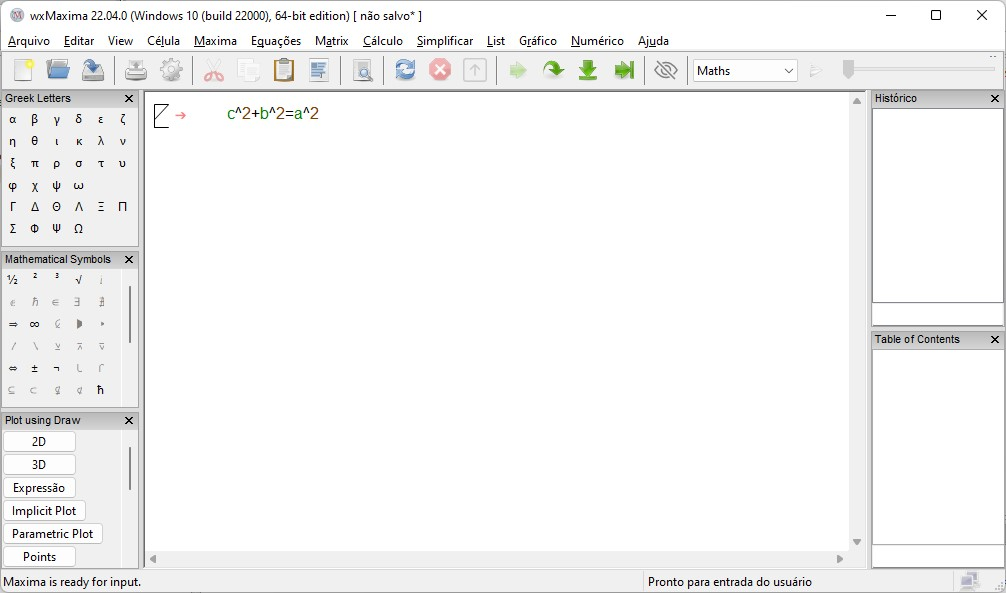
\includegraphics[scale=0.5]{pitagoras.jpg}
	%\end{Center}
\end{figure}

\noindent Essa expressão é o input do processo. O Maxima processará essa entrada após acionada a combinação de tecla \texttt{Shift+Enter} do que, em seguida, apresentará uma saída na área do \emph{prompt}, figura \ref{fig:pitagoras-2}.

\begin{figure}[ht]
    \centering
    \caption{Saída apresentada após após processamento da expressão algébrica entrada.}
        \label{fig:pitagoras-2}
    %\begin{Center}
    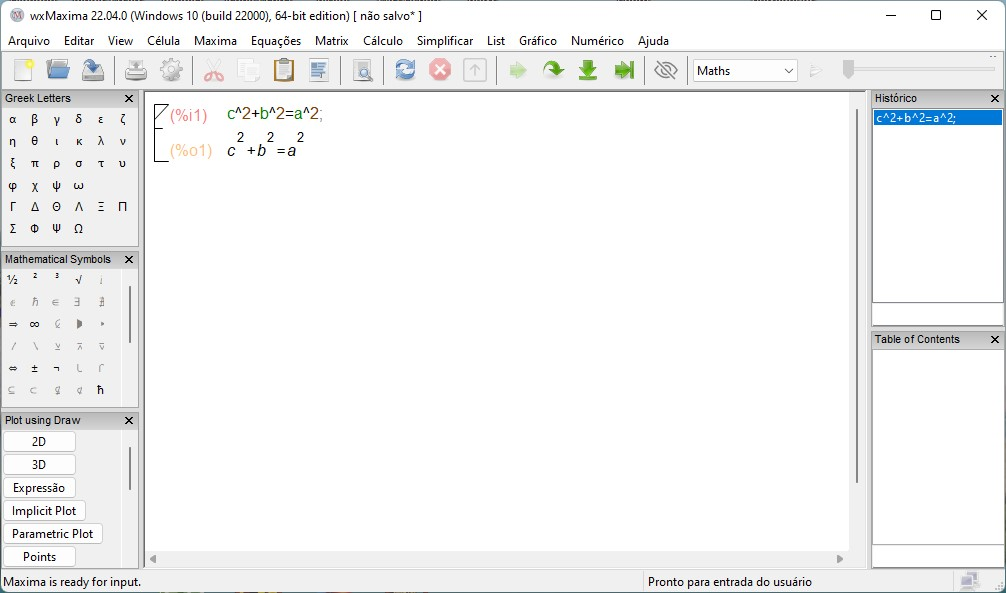
\includegraphics[scale=0.5]{pitagoras-2.jpg}
	%\end{Center}
\end{figure}
\pagebreak
\noindent Observe que a resposta disponibilizada recebe identificadores, tais que:

\begin{minipage}[]{4.000000em}\color{red}\bfseries (\% i1)	
\end{minipage}, indica que a expressão na linha é o \emph{input}, e 

%%%%

\begin{minipage}[]{4.000000em}\color{green}\bfseries (\% o1)	
\end{minipage}, indica que a expressao na linha é a saída (\emph{output}).


No Maxima é possível \emph{nomear uma expressão} de forma que possa ser reutilizada. Por exemplo, escrevendo no prompt a seguinte expressão: \textsf{pitg:c\^\ 2+b\^\ 2=a\^\ 2}. Observe o resultado disso na figura \ref{fig:pitagoras-3}.
\begin{figure}[ht]
    \centering
    \caption{Nomeando expressões.}
        \label{fig:pitagoras-3}
    %\begin{Center}
    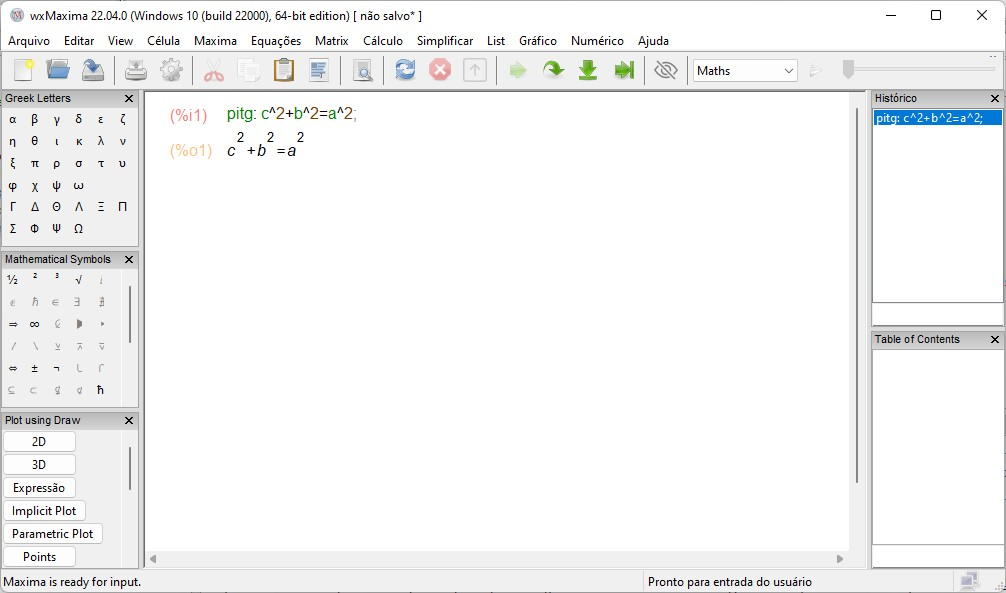
\includegraphics[scale=0.5]{pitagoras-3.jpg}
	%\end{Center}
\end{figure}


\noindent Essa ação de nomear as expressões algébricas é importante pois facilita a reutilização recorrente da fórmula. Por exemplo, com a seguinte expressão nomeada \textsf{sol1:solve(pitg,a)}. O termo \emph{solve} corresponde a uma fórmula (função) interna do Maxima. Os resultados aparecem na figura \ref{fig:pitagoras-4}. 
\begin{figure}[ht!]
    \centering
    \caption{Usando expressões.}
        \label{fig:pitagoras-4}
    %\begin{Center}
    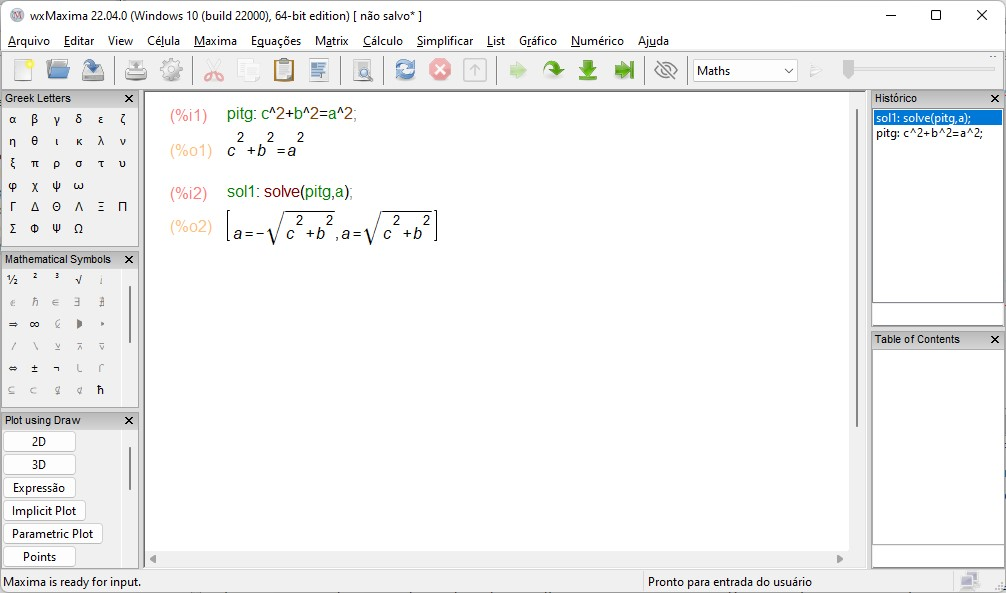
\includegraphics[scale=0.5]{pitagoras-4.jpg}
	%\end{Center}
\end{figure}
%%%

\pagebreak
\noindent Ao aplicar um termo \emph{solve}, o Maxima soluciona a expressão, no caso, \emph{pitg} para a literal \emph{a} tratando-a como a variável incógnita. Observe que o Maxiama retorna dois valores como saída, que era o que seria obtido, caso fossemos desenvolver a solução manualmente, e tais valores são apresentados no formato de uma lista ou vetor linha de dois elementos. 

Uma funcionalidade do Maxima é a possibilidade de recuperar um elemento de um vetor ou lista. Por exemplo, vamos recuperar uma das soluções obtidas do passo anterior. Vamos usar a seguinte sintaxe como \emph{input}: \textsf{sol2:sol1[2];}. O resultado é mostrado na figura \ref{fig:pitagoras-5}
\begin{figure}[ht!]
    \centering
    \caption{Obtendo o valor de um elemento de uma lista.}
        \label{fig:pitagoras-5}
    %\begin{Center}
    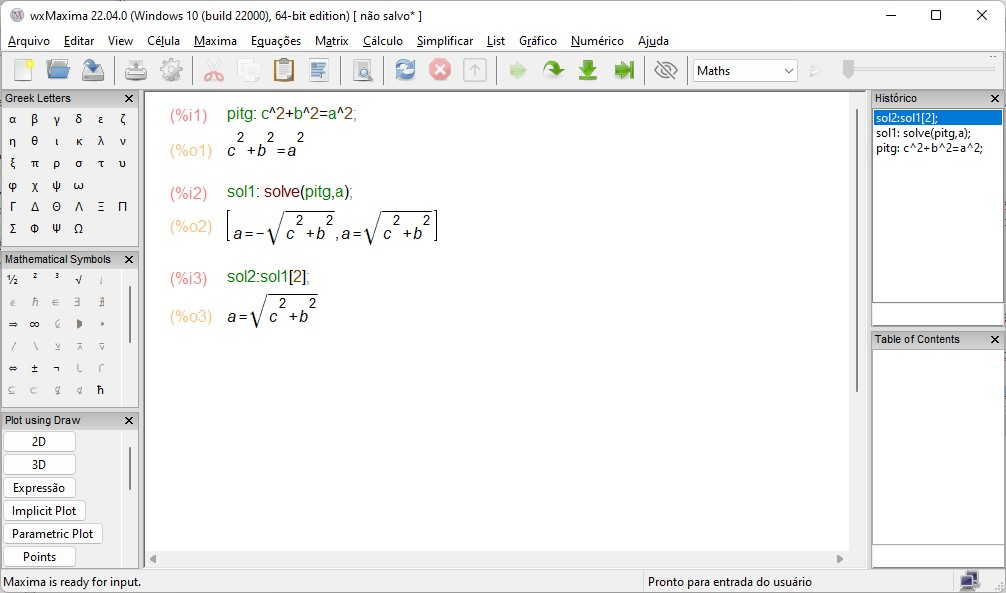
\includegraphics[scale=0.5]{pitagoras-5.jpg}
	%\end{Center}
\end{figure}
%%%

\noindent Observe que o Maxima atribuiu à expressão \textsf{sol2} o valor do segundo elemento do vetor \textsf{sol1}, ou seja, o valor do elemento de índice \textsf{[2]}

O Maxima também suporta um ambiente de texto, misturado entre os comandos algébricos, recurso muito útil no caso de o usuário precisar de documentar seu trabalho com texto explicativo e formatado. Por exemplo vamos colocar um título introdutório em nossa tela e uma texto explicativo intermediário. 

\noindent O título será um texto a ser inserido antes da primeira célula. Uma célula é o espaço delimitado pelo seletor lateral (parentese "exótico" que aparece à esquerda das expressões) idêntico ao desenho abaizo
\begin{figure}[h]
	\centering
		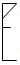
\includegraphics[scale=0.6]{seletor.jpg}
	\label{fig:seletor}
\end{figure}

\noindent O cursor horizontal deve ser transportado com auxílio das teclas de navegação do teclado, ou diretamente com o uso de dispositivo apontador ("mouse"), ver figura \ref{fig:curso-hrizontal-2}. 

\begin{figure*}[hp]
	\centering
	\caption{Posição sugerida para escrever um título}
		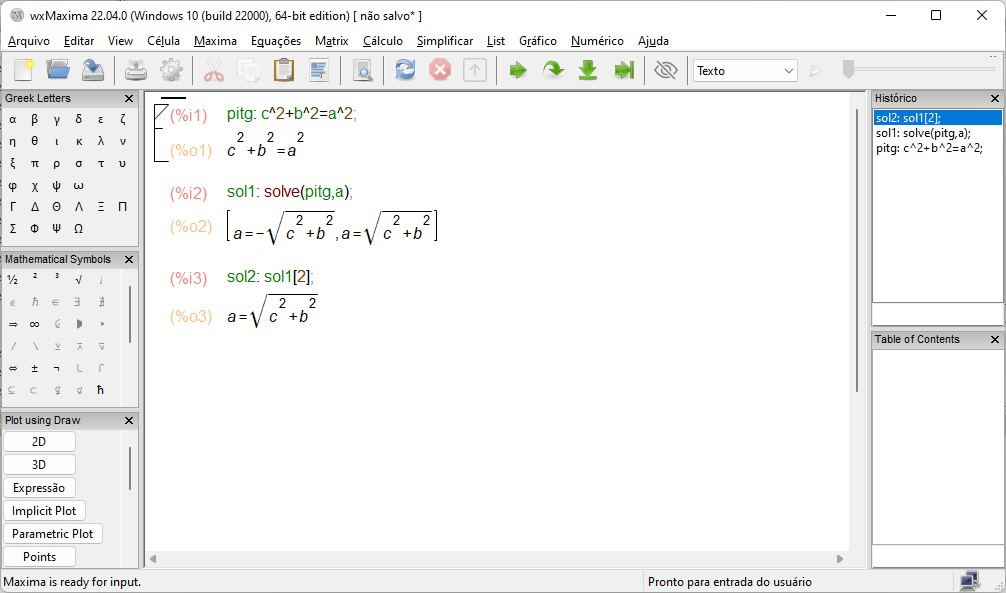
\includegraphics[width=0.80\textwidth]{curso-hrizontal-2.jpg}
	\label{fig:curso-hrizontal-2}
\end{figure*}

Em seguida digita-se o texto pretendido para título:
\begin{figure}[ht!]
	\centering
		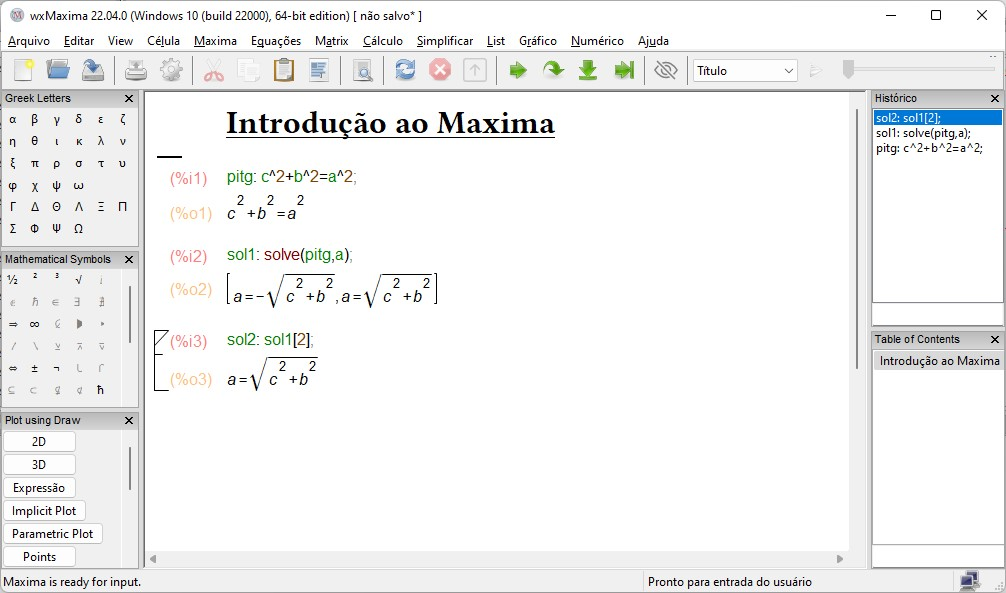
\includegraphics[width=0.80\textwidth]{introducao-maxima.jpg}
	\caption{Resultado da inserção de título}
	\label{fig:introducao-maxima}
\end{figure}
\clearpage

E, digita-se um texto explicativo pretendido:
\begin{figure}[ht!]
	\centering
	\caption{Resultado da inserção de texto comum}
		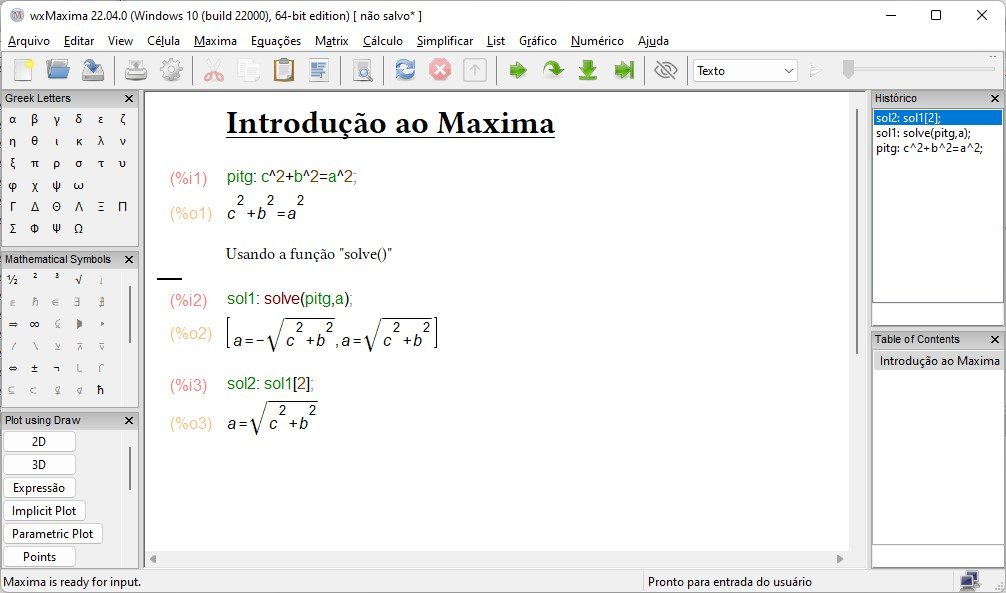
\includegraphics[width=0.80\textwidth]{usando-solve.jpg}
	\label{fig:usando-solve}
\end{figure}
\clearpage
%\pagebreak
Por hora esses são os conhecimentos sobre o Maxima, indispensáveis para imergir sobre o univero de possibildades. São conhecimentos básicos e no decorrer dos outros capítulos estaremos apresentando outos recursos básicos ou mais complexos, conforme a exigência do contexto.
\chapter{ESTUDO DAS FUNÇÕES TRIGONOMÉTRICAS}
\newcounter{exemplos}
\setcounter{exemplos}{1}
\newcounter{exercicios}
\setcounter{exercicios}{1}
As funções trigonométricas tiveram suas origens no estudo das medidas astronômicas, e elas são de suma importância para as ciências em geral, dado que as suas características permitem de serem utilizadas para representar o comportamento de diversos sistemas reais. 

Elas são desenvolvidas por meio do estudo da circunferência de raio unitário com relação às dimensões de determinado sistema de cordas. A palavra \emph{seno} etimologicamente significa meia corda.

As funções trigonométricas também tem relações com a geometria por meio das relações trigonométricas no triângulo retângulo.
\section{As Funções Trigonométricas no Maxima}
No Maxima você irá se referir às funções trigonométricas usando as seguintes sintaxes.
\begin{itemize}
	\item Para seno: \textsf{f(x):=sin(x)};
	\item Para cosseno: \textsf{f(x):=cos(x)};
	\item Para tangente: \textsf{f(x):=tan(x)},
\end{itemize}
onde \emph{x}, ou seja, o argumento de função, deve ser entendido como medida de arco expressa em radianos.

Vamos a uma ilustração. Vamos construir uma tabela dessas funções, para alguns pouco valores de arco.

%%%%%%Matlab
\clearpage
\pagebreak{}
{\large {\scshape Exemplo \thesection.\theexemplos: Construindo uma tabela}}

\noindent
%%%%%%%%
%% INPUT:
\begin{minipage}[t]{4.000000em}\color{red}\bfseries
\ensuremath{\ensuremath{}}	
\end{minipage}
\begin{minipage}[t]{\textwidth}\color{blue}
/*Definição\ das\ funções\ trigonométricas\ no\ ambiente.\ */\\
f(x):=sin(x)\$;\ g(x):=cos(x)\$\ \ \ \ \ \ \ \ \ \ \ \ \ \ \ \ \ \ \ 
\end{minipage}
\\
\noindent%

\noindent
%%%%%%%%
%% INPUT:
\begin{minipage}[t]{4.000000em}\color{red}\bfseries
\ensuremath{\ensuremath{}}	
\end{minipage}	
\begin{minipage}[t]{\textwidth}\color{blue}
/*configuração\ do\ ambiente\ para\ calculos\ simbólicos\ (não\ numérico).\ */\\
numer:false\$\ \ \ \ \ \ \ \ \ \ \ \ \ \ \ \ \ \ \ \ \ \ \\
/*\ inicializa\ incremento\ para\ cálculo\ \ do\ domínio\ de\ valores\ para\ "x".\ */\\
arc:\ensuremath{\pi}/12\ \$\ \ \ \ \ \ \ \ \ \ \ \ \ \ \ \\
\\
\ /*gera\ lista\ com\ os\ elementos\ para\ o\ cabeçalho\ de\ colunas.\ */\\
cabeçalhoDaTabela:\ ["Arco(rad)",\ arc,\ 2*arc,\ 3*arc,\ 4*arc\ ]\$\ \ 
\end{minipage}

\noindent%

\noindent
%%%%%%%%
%% INPUT:
\begin{minipage}[t]{4.000000em}\color{red}\bfseries
\ensuremath{\ensuremath{}}	
\end{minipage}
\begin{minipage}[t]{\textwidth}\color{blue}
/*a\ partir\ daqui\ o\ cálculo\ será\ numérico.\ */\\
numer:\ true\$\ \ \ \ \ \ \ \ \ \ \ \ \ \ \ \ \ \ \ \ \ \ \ \ \ \ \ \ \ \ \ \ \ \ \ \ \ \ \ \ \ \ \ \ \ \ \ \ \ \ \ \ \ \ \ \ \ \ \ \ \ \ \ \\
arc:\ensuremath{\pi}/12\ \$
\end{minipage}
\\
\noindent%

\noindent
%%%%%%%%
%% INPUT:
\begin{minipage}[t]{4.000000em}\color{red}\bfseries
\ensuremath{\ensuremath{}}	
\end{minipage}
\begin{minipage}[t]{\textwidth}\color{blue}
\ /*construindo\ lista\ de\ valores\ de\ seno.\ */\\
linha1:makelist(f(x),x,\ [arc,2*arc,3*arc,4*arc])\$\ \ \ \ \ \ \ \ \ \ \ \ \\
/*a\ lista\ é\ reconstruída\ para\ incluir\ nela\ um\ cabeçalho\ de\ linha.\ */\\
linha1:["Seno",\ linha1[1],\ linha1[2],\ linha1[3],\ linha1[4]]\$\ \ \ \ \ 
\end{minipage}
\\
\noindent%

\noindent
%%%%%%%%
%% INPUT:
\begin{minipage}[t]{4.000000em}\color{red}\bfseries
\ensuremath{\ensuremath{}}	
\end{minipage}
\begin{minipage}[t]{\textwidth}\color{blue}
\ /*construindo\ lista\ de\ valores\ de\ cosseno.\ */\\
linha2:makelist(g(x),x,\ [arc,2*arc,3*arc,4*arc])\$\ \ \ \ \ \ \ \ \ \ \\
/*a\ lista\ é\ reconstruída\ para\ incluir\ nela\ um\ cabeçalho\ de\ linha.\ */\\
linha2:["Cosseno",linha2[1],\ linha2[2],\ linha2[3],\ linha2[4]]\$\ \ 
\end{minipage}
\\
\noindent%

\noindent
%%%%%%%%
%% INPUT:
\begin{minipage}[t]{4.000000em}\color{red}\bfseries
    \ensuremath{\ensuremath{}}	
\end{minipage}
\begin{minipage}[t]{\textwidth}\color{blue}
    \ /*----\ Saída\ dos\ Resultados\ ---------------------------------*/\\
\end{minipage}
\noindent%


\noindent
%%%%%%%%
%% INPUT:
\begin{minipage}[t]{4.000000em}\color{red}\bfseries
    \ensuremath{\ensuremath{}}	
\end{minipage}
\begin{minipage}[t]{\textwidth}\color{blue}
    \ /*definindo\ a\ precisão\ numérica.\ */\\
fpprintprec\ :\ 3\$\ \ \ \ \ \ \ \ \ \ \ \ \ \ \ \ \ \ \ \ \ \ \ \ \ \ \ \ \ \ \ \ \ \ \ \ \ \ \ \ \ \ \ \ \ \ \ \ \ \ \ \ \ \ \ \ \ \ \ \ \ \ \ \ \ \ \ \ 
\end{minipage}
\\
\noindent%


\noindent
%%%%%%%%
%% INPUT:
\begin{minipage}[t]{4.000000em}\color{red}\bfseries
    \ensuremath{\ensuremath{}}	
\end{minipage}
\begin{minipage}[t]{\textwidth}\color{blue}
    /*formato\ usando\ a\ função\ table\_form().\ \ */\\
    table\_form([cabeçalhoDaTabela,\ linha1,\ linha2]);\ \ \ \ \ 
\end{minipage}
\\
\noindent%


\noindent
%%%%%%%%
%% INPUT:
\begin{minipage}[t]{4.000000em}\color{red}\bfseries
    \ensuremath{\ensuremath{}}	
\end{minipage}
\begin{minipage}[t]{\textwidth}\color{blue}
    /*formato\ usando\ a\ função\ matrix().\ \ */\\
    matrix(cabeçalhoDaTabela,\ linha1,\ linha2);\ \ \ \ \ \ \ \ \ \ \ \ \ \ \ \ \ \ \ \ \ \ 
\end{minipage}
%%
% 
% $$e^{\pi i} + 1 = 0$$
% 
%%%%%%

Copie na memória do seu computador as linhas de comando desse exemplo e cole na janela do wxMaxima, avalie com o comando de teclado \texttt{Shift+Enter} e veja o resultado, deverá ser idêntico ao da figura \ref{fig:exemplo331}
\begin{figure}[H]
    \centering
    \caption{Resultado do exemplo na janela do wxMaxima.}
        \label{fig:exemplo331}
    %\begin{Center}
    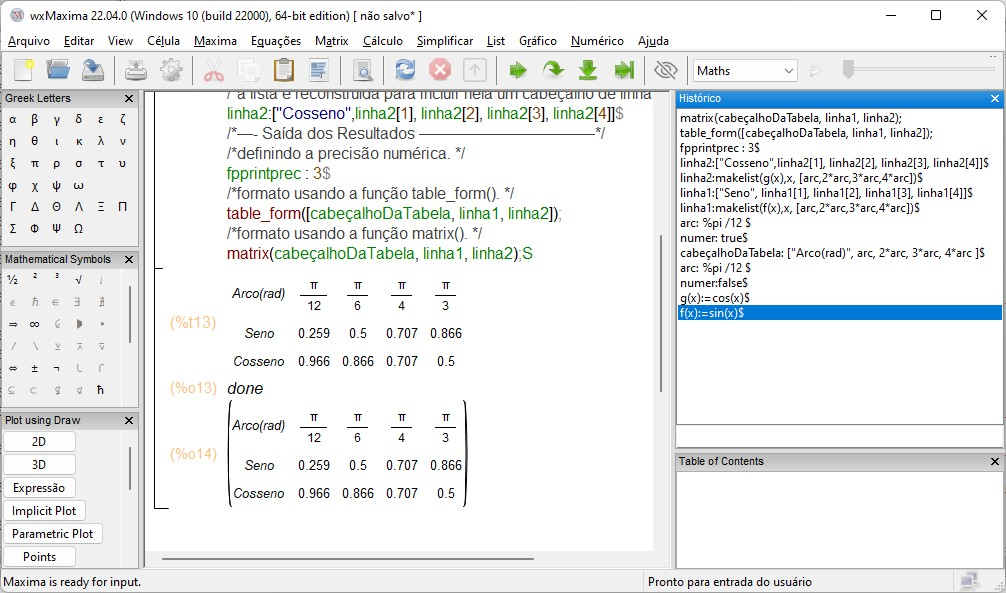
\includegraphics[scale=0.6]{exemplo331.jpg}
	%\end{Center}
\end{figure}
\vspace{20pt}
%%% pesquisar evfun no maxima  - distribute_over	- cabs - Trigonometric functions
%%%
\begin{tcolorbox}[enhanced jigsaw, colback=gray!30, colframe=Maroon,width=1\textwidth, arc=3mm, auto outer arc, boxrule=5pt, drop shadow={Maroon!50!gray!80}]
  	\noindent
	Exercício \thesection.\theexercicios: No encejo do exemplo \thesection.\theexemplos, acrescente ou modifique comando de forma que apareçam, uma linha correspondente aos valores de tangente e uma coluna correspondente ao arco igual a $\frac{5\,\pi}{12}$.
\end{tcolorbox}
%%%
\section{Manipulando Expressões Trigonométrica}
Esta seção será dedicada a mostrar como trabalhar expressões trigonométricas no Maxima.
\subsubsection{Soma de Arcos}
usa-se a função: \texttt{trigexpand}.

\section{Construção de Gráficos}

\chapter{DICAS SOBRE O MAXIMA}
\begin{itemize}
	\item Se seu cálculo está demorando de mais para executar, você pode tentar os menus 'Maxima->Interromper' ou 'Maxima->Reiniciar o Maxima'.
	\item Para fazer gráficos em coordenadas polares, selecione 'Polar' em Opções na janela de gráficos bidimensionais. Você também pode fazer gráficos em coordenadas esféricas e cilíndricas em 3D.
	\item As janelas do wxMaxima têm valores padrão para as entradas, um dos quais é '\%'. Se você selecionou algo no documento, a seleção será usada no lugar de '\%'.
	\item Ao aplicar funções com um argumento a partir dos menus, o argumento padrão é '\%'. Para aplicar a função a um outro valor, selecione-o do documento antes de executar o comando do menu.
	\item Para salvar o tamanho e posição da janela do wxMaxima entre sessões, use a janela 'Maxima->Configurações'.
	\item Você pode acessar a última saída com a variável '\%'. Você pode acessar a saída de comandos anteriores usando a variável '\%on' onde n é o número da saída.
	\item Células de título, seção e subseção podem ser recolhidas para ocultar seu conteúdo. Para recolher ou expandir, clique no quadrado próximo à celula. Se você segurar Shift enquanto clica, todos os subníveis daquela célula também serão recolhidos/expandidos.
	\item Você pode esconder a saída das células clicando no triângulo no lado esquerdo das células. Isso funciona também em células de texto.
	\item Um 'cursor horizontal' foi introduzido no wxMaxima 0.8.0. Ele é mostrado como uma linha horizontal entre células. Ele mostra onde uma nova célula vai aparecer se você digitar ou colar texto, ou se executar um comando do menu.
	\item O cursor horizontal funciona como um cursor normal, mas ele opera em células: pressione as setas para cima ou para baixo para movê-lo; segure Shift enquanto move para selecionar células; pressione Backspace ou Delete duas vezes apaga a célula próxima ao cursor.
	\item Você pode selecionar vários células com o mouse - clique e arraste desde algum ponto entre células ou dos marcadores à esquerda - ou com o teclado - segure Shift enquanto move o cursor horizontal - e então operar na seleção. Isso é útil quando você quer apagar ou calcular múltiplas células.
	\item Você pode avaliar todo o documento usando o menu 'Célula->Avaliar todas as células' ou a tecla de atalho correspondente. As células serão avalidas na ordem em que aparecem no documento.
	\item As janelas do wxMaxima têm valores padrão para as entradas, um dos quais é '\%'. Se você selecionou algo no documento, a seleção será usada no lugar de '\%'.
	\item Equations have several advantages over functions. For example they can be manipulated with factor(), expand() and similar functions. They can easily be introduced one into another. Also they are always printed out as 2D maths.
\end{itemize}
\section{Dicas de Maxima}
Maxima's strengths are manipulating equations and in symbolic calculations. It therefore makes sense to use functions (as opposed to equations with labels) sparingly and to keep the actual values of variables in a list, instead of directly assigning them values. An example session that does do so would be:
\begin{verbatim}
/* We keep the actual values in a list so we can use them later on */
    Values:[a=10,c=100];
    Pyth:a^2+b^2=c^2;
    solve(%,b);
    result:%[2];
    at(result,Values);
    float(%);
\end{verbatim}
Maxima's "at" function allows to access to arbitrary variables in a list of results:
\begin{verbatim}
    g1:a*x+y=0;
    g2:b*y+x*x=1;
    solve([g1,g2],[a,b]);
    %[1];
    result_b:b=at(b,%);
\end{verbatim}

\end{document}